\chapter{Giới thiệu}
\label{chap:chap1-introduce}

Tại chương này, tác giả giới thiệu cấu trúc thư mục của dự án, giải thích các cài đặt, một số lưu ý trong quá trình sử dụng. Chương này cũng như báo cáo này không giới thiệu các cú pháp cơ bản như gõ phương trình, tạo bảng đơn giản, chèn hình ảnh.

\section{Cấu trúc thư mục}

\indent Hình \ref{fig:chap1-project-directory} mô tả cấu trúc thư mục của dự án. Thư mục \textbf{chapters} lưu các thành phần văn bản chính của dự án. Trong thư mục này chia làm ba thư mục, \textbf{\textit{back}} tương ứng với các phụ lục phía sau báo cáo.

\begin{figure}
    \centering
    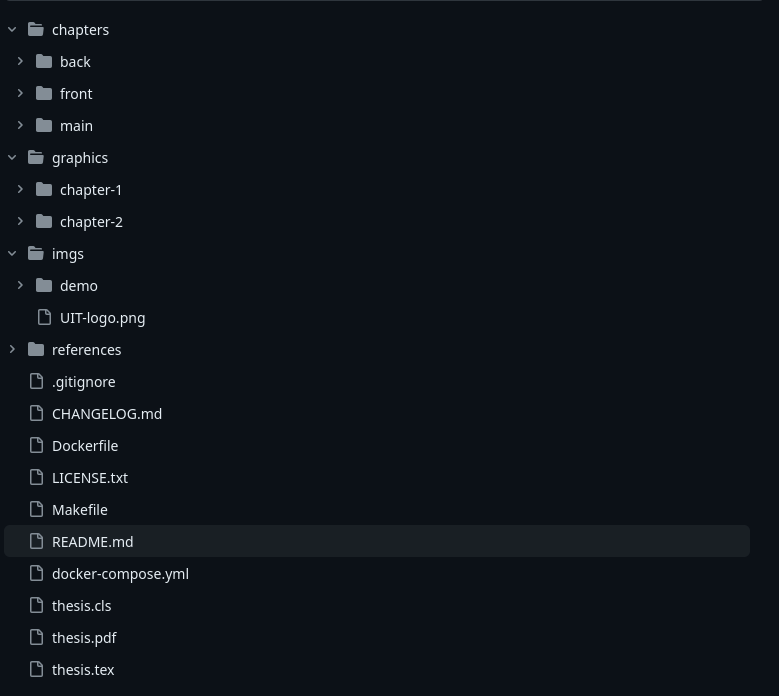
\includegraphics[scale=0.5]{chapter1/chap1-project-directory.png}
    \caption{Cấu trúc thư mục của dự án}
    \label{fig:chap1-project-directory}
\end{figure}

Thư mục \textbf{\textit{front}} tương ứng với các trang thông tin hội đồng chấm tốt nghiệp, lời cảm ơn, danh mục từ viết tắt... Thư mục \textbf{\textit{main}} chứa các chương của báo cáo. Báo cáo đánh số thứ tự riêng cho phần \textit{\textbf{front}}, trong khi phần các chương chính và phần phụ lục được đánh số giống nhau. Báo cáo đánh số trang bắt đầu từ trang tóm tắt, chữ số Ả-rập, bắt đầu bằng 1.

Thư mục \textbf{\textit{graphics}} chứa hình ảnh được chèn vào báo cáo. Tương ứng với mỗi chương sẽ có 1 thư mục hình ảnh của chương đó.

Thư mục \textbf{\textit{imgs}} là thư mục chứa hình ảnh của dự án, nó bao gồm các logo, watermark hoặc hình ảnh phục vụ cho document trên github. Hình chèn vào báo cáo không được lưu trong thư mục này.

Thư mục \textbf{\textit{references}} chứa các file chỉ mục tài liệu tham khảo. Tương tự như mỗi chapter một file .tex, nó cũng có riêng một file .bib để chỉ rõ các tài liệu tham khảo nào được sử dụng trong chuong nào.

File \textbf{\textit{thesis.cls}} là file quy định các câu lệnh, mức chỉ mục đánh số hình ảnh, bảng biểu, phần, chương. Quy định header và footer, trang  bìa.... Chi tiết xem trong file. Hãy chắc chắn rằng bạn hiểu rõ tất cả nếu muốn thay đổi gì trong file này.

File \textbf{\textit{thesis.tex}} là file quy định cấu trúc báo cáo, chương nào trước, chương nào sau, quy định thư mục hình ảnh chèn trong báo cáo. Nó quy định thông tin người báo cáo thông qua các câu lệnh được quy định trong file .cls. 